\documentclass[preprint,12pt,aps,pra,showkeys,amsmath,amssymb,superscriptaddress,floatfix]{revtex4-2}
\usepackage[T1]{fontenc}
\usepackage[utf8]{inputenc}
\usepackage{amsmath,amssymb,amsthm,mathtools,mathrsfs}
\usepackage{microtype,booktabs,enumitem}
\usepackage{xcolor,tikz,etoolbox}
\usepackage[skins,breakable]{tcolorbox}
\usepackage{needspace}
% Keep diagram geometry independent of REVTeX preprint body spacing.
\AtBeginEnvironment{tikzpicture}{\linespread{1}\selectfont}
\usetikzlibrary{arrows.meta,positioning,calc,fit,decorations.pathreplacing}
\usepackage{graphicx}
\usepackage{hyperref}

\definecolor{MMBlue}{RGB}{0,82,155}
\definecolor{MMOrange}{RGB}{200,80,0}
\tikzset{
 mmnode/.style={draw=MMBlue,rounded corners=2pt,fill=MMBlue!4,align=left,execute at begin node={\raggedright},text width=5cm,font=\fontsize{10}{12}\selectfont,inner sep=6pt},
 mmimport/.style={mmnode,draw=black!65,fill=black!4},
 mmcandidate/.style={mmnode,draw=MMOrange,dashed,fill=MMOrange!5},
 mmrejected/.style={mmnode,draw=black,densely dotted,fill=black!8},
 mmproof/.style={->,thick,MMBlue},
 mmflow/.style={->,semithick,black!70},
 mmrepair/.style={->,dashed,thick,MMOrange},
 mmcandidatearrow/.style={->,dashed,semithick,MMOrange},
 mmnote/.style={font=\scriptsize,fill=white,inner sep=2pt,align=center}}

\usepackage[section]{placeins}
\setlength{\emergencystretch}{3em}
\setlist{itemsep=3pt,topsep=4pt}
\newtheorem{theorem}{Theorem}[section]
\newtheorem{proposition}[theorem]{Proposition}
\newtheorem{lemma}[theorem]{Lemma}
\newtheorem{corollary}[theorem]{Corollary}
\theoremstyle{definition}
\newtheorem{definition}[theorem]{Definition}
\newtheorem{example}[theorem]{Example}
\theoremstyle{remark}
\newtheorem{remark}[theorem]{Remark}
% Avoid isolated statement headings and single-line paragraph fragments.
\BeforeBeginEnvironment{theorem}{\Needspace{6\baselineskip}}
\BeforeBeginEnvironment{definition}{\Needspace{5\baselineskip}}
\BeforeBeginEnvironment{proposition}{\Needspace{5\baselineskip}}
\BeforeBeginEnvironment{lemma}{\Needspace{5\baselineskip}}
\BeforeBeginEnvironment{corollary}{\Needspace{5\baselineskip}}
\clubpenalty=5000
\widowpenalty=5000
\newcommand{\R}{\mathbb R}\newcommand{\Z}{\mathbb Z}\newcommand{\N}{\mathbb N}
\newcommand{\Pa}{\operatorname{Pa}}\newcommand{\Desc}{\operatorname{Desc}}
\newcommand{\cl}{\operatorname{cl}}\newcommand{\cost}{\operatorname{cost}}
\newcommand{\status}{\operatorname{status}}
% Faculty cards: a visual rail groups the five faculties within one agent.
% The rail has no arrowhead and does not represent a proof dependency.
\newcommand{\mmfacultybadge}[1]{%
 \node[circle,draw=MMBlue,line width=1pt,fill=white,
 minimum size=7mm,inner sep=0pt,font=\sffamily\small\bfseries,text=MMBlue]
 at ([xshift=15pt,yshift=-15pt]frame.north west) {#1};}
\newcommand{\mmfacultyrail}{%
 \draw[MMBlue!80,line width=1pt]
 ([xshift=15pt,yshift=2pt]frame.north west)--
 ([xshift=15pt,yshift=-2pt]frame.south west);}
\newtcolorbox{mmfacultybox}[2]{enhanced,breakable,
 colback=MMBlue!4,colframe=MMBlue!4,boxrule=0pt,arc=3pt,
 left=39pt,right=9pt,top=4pt,bottom=4pt,
 before skip=2pt,after skip=2pt,
 fontupper=\small\linespread{1.1}\selectfont,
 overlay unbroken={\mmfacultyrail\mmfacultybadge{#1}},
 overlay first={\mmfacultyrail\mmfacultybadge{#1}},
 overlay middle={\mmfacultyrail},overlay last={\mmfacultyrail}}
\newcommand{\mmfaculty}[3]{%
 \begin{mmfacultybox}{#1}{#2}
 {\sffamily\bfseries\color{MMBlue}#2}\par\smallskip #3
 \end{mmfacultybox}}
\newcommand{\agent}[9]{%
 \Needspace{8\baselineskip}
 \subsubsection{#1}
 \noindent\textbf{Object.} #2\par
 \noindent\textbf{Role.} #3\par\smallskip
 \mmfaculty{E}{Ego}{#4}
 \mmfaculty{M}{Memory}{#5}
 \mmfaculty{I}{Intellect}{#6}
 \mmfaculty{S}{Sense}{#7}
 \mmfaculty{A}{Action}{#8}
 \smallskip\noindent #9\par}

\usepackage{longtable,array,calc}
\providecommand{\tightlist}{\setlength{\itemsep}{2pt}\setlength{\parskip}{0pt}}
\makeatletter
\def\frontmatter@abstract@produce{\par\addvspace{\frontmatter@preabstractspace}%
\begingroup\prep@absbox\unvbox\absbox\post@absbox\endgroup
\addvspace{\frontmatter@postabstractspace}}
\makeatother
\newcommand{\field}[2]{\par\smallskip\noindent\textbf{#1.} #2\par}
\setlength{\emergencystretch}{5em}
\AtBeginEnvironment{verbatim}{\small\linespread{1.0}\selectfont}


\hypersetup{colorlinks=true,linkcolor=MMBlue,urlcolor=MMBlue,pdfauthor={Dibakar Sigdel}}

\begin{document}

\title{Fundamental Group of the Torus via Seifert--van Kampen\\[4pt]\large An End-to-End Meta-Math Walkthrough}

\author{Dibakar Sigdel}

\affiliation{Mindverse Computing LLC, Lynnwood, WA 98087, USA}

\date{October 2026}

\begin{abstract}

A complete authored walkthrough of fundamental group of the torus via
seifert--van kampen, with explicit mathematical contracts, local
verification gates, and reusable exports. The report presents the target
theorem, declared imports, a dependency graph, five-faculty node
contracts, a continuous proof, a worked example, and a hypothesis-repair
audit. It is an authored mathematical exposition, not a deployed-agent
transcript or a formal proof-assistant certificate.

\end{abstract}\maketitle\linespread{1.12}\selectfont

\noindent\textbf{AT-02 / Algebraic Topology / Report v1}

\section{Target and import contract}

\begin{theorem}

For the torus \(T^2\), prove

\[\pi_1(T^2)\cong\langle a,b\mid aba^{-1}b^{-1}=1\rangle\cong\mathbb Z^2.\]

The output is a fundamental-group presentation followed by an explicit
group isomorphism. A drawing of two loops or the assertion that they
commute is not a proof that these are all generators and relations.

\end{theorem}

\subsection{Foundations and permitted imports}

a based loop is considered modulo based homotopy; multiplication is loop
concatenation. Import \(\pi_1(S^1)\cong\mathbb Z\), homotopy invariance,
and Seifert--van Kampen for path-connected open sets with path-connected
intersection. For such a cover, the theorem gives the group pushout:
relations identify the two images of the intersection group. We
explicitly construct the cover used for the torus's two-cell attachment.

\clearpage\section{Node interaction workflow}

\begin{center}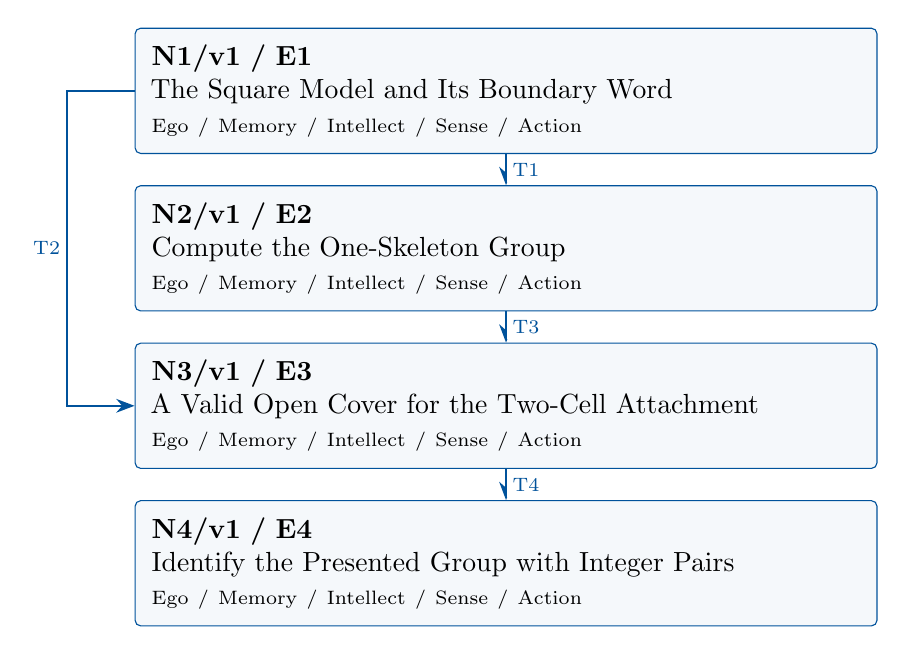
\begin{tikzpicture}[>=Stealth,x=1cm,y=1cm]

\node[mmnode,text width=9cm,minimum height=1.25cm] (N1) at (0,0.0) {\textbf{N1/v1 / E1}\\The Square Model and Its Boundary Word\\{\scriptsize Ego / Memory / Intellect / Sense / Action}};

\node[mmnode,text width=9cm,minimum height=1.25cm] (N2) at (0,-2.0) {\textbf{N2/v1 / E2}\\Compute the One-Skeleton Group\\{\scriptsize Ego / Memory / Intellect / Sense / Action}};

\node[mmnode,text width=9cm,minimum height=1.25cm] (N3) at (0,-4.0) {\textbf{N3/v1 / E3}\\A Valid Open Cover for the Two-Cell Attachment\\{\scriptsize Ego / Memory / Intellect / Sense / Action}};

\node[mmnode,text width=9cm,minimum height=1.25cm] (N4) at (0,-6.0) {\textbf{N4/v1 / E4}\\Identify the Presented Group with Integer Pairs\\{\scriptsize Ego / Memory / Intellect / Sense / Action}};

\draw[mmproof] (N1.south) -- node[mmnote,right] {T1} (N2.north);

\draw[mmproof] (N1.west) -- (-5.58,0) -- node[mmnote,left] {T2} (-5.58,-4) -- (N3.west);

\draw[mmproof] (N2.south) -- node[mmnote,right] {T3} (N3.north);

\draw[mmproof] (N3.south) -- node[mmnote,right] {T4} (N4.north);

\end{tikzpicture}\end{center}

Each box is one mathematical agent containing all five faculties. Blue
arrows carry the versioned exports listed below. The layout gives a
reading order; only drawn arrows assert dependencies. Diagnostic repair
is separate from the proof DAG.

\clearpage\subsection{Versioned evidence-transfer ledger}

\begingroup\small\linespread{1.05}\selectfont

\Needspace{5\baselineskip}\field{T1: N1/E1/v1 to N2}{The torus has one vertex, loops \(a,b\), and one two-cell attached by
\(aba^{-1}b^{-1}\).}

\field{Receiving activity}{N2: Compute the One-Skeleton Group}

\field{Compatibility}{Use the same mathematical objects and hypotheses as the source export.
Receiving contract: N1/E1, the circle group, and Seifert--van Kampen.}

\Needspace{5\baselineskip}\field{T2: N1/E1/v1 to N3}{The torus has one vertex, loops \(a,b\), and one two-cell attached by
\(aba^{-1}b^{-1}\).}

\field{Receiving activity}{N3: A Valid Open Cover for the Two-Cell Attachment}

\field{Compatibility}{Use the same mathematical objects and hypotheses as the source export.
Receiving contract: N1/E1, N2/E2, and van Kampen with a valid open
cover.}

\Needspace{5\baselineskip}\field{T3: N2/E2/v1 to N3}{The one-skeleton has fundamental group \(F(a,b)\).}

\field{Receiving activity}{N3: A Valid Open Cover for the Two-Cell Attachment}

\field{Compatibility}{Use the same mathematical objects and hypotheses as the source export.
Receiving contract: N1/E1, N2/E2, and van Kampen with a valid open
cover.}

\Needspace{5\baselineskip}\field{T4: N3/E3/v1 to N4}{\(\pi_1(T^2)=F(a,b)/\langle\!\langle aba^{-1}b^{-1}\rangle\!\rangle\).}

\field{Receiving activity}{N4: Identify the Presented Group with Integer Pairs}

\field{Compatibility}{Use the same mathematical objects and hypotheses as the source export.
Receiving contract: N3/E3 and the universal property of a group
presentation.}

\endgroup

\clearpage\section{Agent roles and five-faculty activities}\begingroup\small\linespread{1.05}\selectfont\setlist{itemsep=1pt,topsep=2pt}

\subsection{N1/v1: The Square Model and Its Boundary Word}

\field{Object and role}{The Square Model and Its Boundary Word. Establish the following local
result: The torus has one vertex, loops \(a,b\), and one two-cell
attached by \(aba^{-1}b^{-1}\).}

\field{Inputs}{The quotient square with opposite edges consistently identified.}

\mmfaculty{E}{Ego}{Own E1/v1: The torus has one vertex, loops \(a,b\), and one two-cell
attached by \(aba^{-1}b^{-1}\).}

\mmfaculty{M}{Memory}{Quotient square and orientations}

\mmfaculty{I}{Intellect}{Separate one-skeleton and face}

\mmfaculty{S}{Sense}{Identify all four vertices}

\mmfaculty{A}{Action}{Carry out the numbered deductions and publish E1/v1 together with its
hypotheses and proof location.}

\smallskip\noindent\textbf{Numbered mathematical activities}

\begin{enumerate}[label=N1.\arabic*,leftmargin=3.4em]

\item Track all four vertices to the common vertex.

\item Choose positive horizontal and vertical loop orientations.

\item Read the counterclockwise boundary word with its inverse edges.

\end{enumerate}

\field{Export E1/v1}{The torus has one vertex, loops \(a,b\), and one two-cell attached by
\(aba^{-1}b^{-1}\).}

\field{Acceptance gate}{Identify all four vertices Publish only after checking every displayed
deduction.}

\field{Targeted repair}{If the check fails, revise N1: Identify all four vertices Recheck
dependent nodes N2, N3, N4.}

\clearpage

\subsection{N2/v1: Compute the One-Skeleton Group}

\field{Object and role}{Compute the One-Skeleton Group. Establish the following local result:
The one-skeleton has fundamental group \(F(a,b)\).}

\field{Inputs}{N1/E1, the circle group, and Seifert--van Kampen.}

\mmfaculty{E}{Ego}{Own E2/v1: The one-skeleton has fundamental group \(F(a,b)\).}

\mmfaculty{M}{Memory}{Circle group and van Kampen}

\mmfaculty{I}{Intellect}{Use wedge-of-circles cover}

\mmfaculty{S}{Sense}{Do not assume a and b commute}

\mmfaculty{A}{Action}{Carry out the numbered deductions and publish E2/v1 together with its
hypotheses and proof location.}

\smallskip\noindent\textbf{Numbered mathematical activities}

\begin{enumerate}[label=N2.\arabic*,leftmargin=3.4em]

\item Use two open sets retracting to the individual circles.

\item Check their intersection is a contractible tree.

\item The pushout is the free product \(\mathbb Z*\mathbb Z\), before imposing
a face relation.

\end{enumerate}

\field{Export E2/v1}{The one-skeleton has fundamental group \(F(a,b)\).}

\field{Acceptance gate}{Do not assume a and b commute Publish only after checking every
displayed deduction.}

\field{Targeted repair}{If the check fails, revise N2: Do not assume a and b commute Recheck
dependent nodes N3, N4.}

\clearpage

\subsection{N3/v1: A Valid Open Cover for the Two-Cell Attachment}

\field{Object and role}{A Valid Open Cover for the Two-Cell Attachment. Establish the following
local result:
\(\pi_1(T^2)=F(a,b)/\langle\!\langle aba^{-1}b^{-1}\rangle\!\rangle\).}

\field{Inputs}{N1/E1, N2/E2, and van Kampen with a valid open cover.}

\mmfaculty{E}{Ego}{Own E3/v1:
\(\pi_1(T^2)=F(a,b)/\langle\!\langle aba^{-1}b^{-1}\rangle\!\rangle\).}

\mmfaculty{M}{Memory}{Open-cover pushout}

\mmfaculty{I}{Intellect}{Fill the two-cell}

\mmfaculty{S}{Sense}{Check open sets and connected intersection}

\mmfaculty{A}{Action}{Carry out the numbered deductions and publish E3/v1 together with its
hypotheses and proof location.}

\smallskip\noindent\textbf{Numbered mathematical activities}

\begin{enumerate}[label=N3.\arabic*,leftmargin=3.4em]

\item Take the complement of the face center and a small open disk around that
center.

\item The punctured overlap is path connected; its generator maps to the
attaching word and to the identity respectively.

\item Form the normal closure relation, including the basepoint conjugation.

\end{enumerate}

\field{Export E3/v1}{\(\pi_1(T^2)=F(a,b)/\langle\!\langle aba^{-1}b^{-1}\rangle\!\rangle\).}

\field{Acceptance gate}{Check open sets and connected intersection Publish only after checking
every displayed deduction.}

\field{Targeted repair}{If the check fails, revise N3: Check open sets and connected
intersection Recheck dependent nodes N4.}

\clearpage

\subsection{N4/v1: Identify the Presented Group with Integer Pairs}

\field{Object and role}{Identify the Presented Group with Integer Pairs. Establish the following
local result: \(\pi_1(T^2)\cong\mathbb Z^2\).}

\field{Inputs}{N3/E3 and the universal property of a group presentation.}

\mmfaculty{E}{Ego}{Own E4/v1: \(\pi_1(T^2)\cong\mathbb Z^2\).}

\mmfaculty{M}{Memory}{Presentations and integer pairs}

\mmfaculty{I}{Intellect}{Construct inverse group maps}

\mmfaculty{S}{Sense}{Prove no additional hidden relations}

\mmfaculty{A}{Action}{Carry out the numbered deductions and publish E4/v1 together with its
hypotheses and proof location.}

\smallskip\noindent\textbf{Numbered mathematical activities}

\begin{enumerate}[label=N4.\arabic*,leftmargin=3.4em]

\item Map \(a,b\) to the standard integer coordinate vectors.

\item Define the reverse map \((m,n)\mapsto a^mb^n\), using commutativity.

\item Check both composites are identities, ruling out further integer
relations.

\end{enumerate}

\field{Export E4/v1}{\(\pi_1(T^2)\cong\mathbb Z^2\).}

\field{Acceptance gate}{Prove no additional hidden relations Publish only after checking every
displayed deduction.}

\field{Targeted repair}{If the check fails, revise N4: Prove no additional hidden relations
Withhold this terminal result until its gate passes.}

\endgroup\clearpage\section{Continuous mathematical proof}\label{sec:proof}

\subsection{N1 --- The Square Model and Its Boundary
Word}\label{n1-the-square-model-and-its-boundary-word}

Represent the torus by a square with opposite edges identified in the
same direction. All four vertices become one vertex, and the horizontal
and vertical edge pairs become loops a and b. The one-skeleton Y is the
wedge \(S^1\vee S^1\).

The remaining open square is one two-cell. Traversing its boundary
counterclockwise gives horizontal a, vertical b, reverse horizontal
\(a^{(-1)}\), and reverse vertical \(b^{(-1)}\). Hence its attaching
loop is

\[w=aba^{-1}b^{-1}.\]

Changing consistent orientation conventions can invert or conjugate the
word without changing its normal closure. Inconsistent conventions,
however, can produce the wrong space.

\subsection{N2 --- Compute the One-Skeleton
Group}\label{n2-compute-the-one-skeleton-group}

Cover the wedge by one open set containing the entire first circle and
short arcs around the wedge point on the second, and a second set with
the roles reversed. Each deformation retracts onto its full circle.
Their intersection is a small cross-shaped tree around the common
vertex, which is contractible and path connected.

Van Kampen therefore gives

\[\pi_1(Y)\cong\mathbb Z*\mathbb Z=F(a,b),\]

the free group on a and b. Before the face is filled, the generators do
not commute; the commutator is a nontrivial reduced word in this free
group.

\subsection{N3 --- A Valid Open Cover for the Two-Cell
Attachment}\label{n3-a-valid-open-cover-for-the-two-cell-attachment}

Write X for Y with the closed disk attached along w; this is the square
model of the torus. Choose an interior center o of the attached disk.

Let \(U=X\setminus\{o\}\). This is open and deformation retracts onto Y:
radially push each point in the punctured disk toward its boundary while
fixing Y. Let V be a smaller open disk around o lying wholly inside the
two-cell. It is open and contractible. These sets cover X. Their
intersection is a punctured smaller disk, path connected, with
fundamental group Z.

Choose a basepoint in that intersection and a path in U to the original
vertex. A positive generator of the intersection group, transported to Y
by the radial retraction, becomes w up to this basepoint conjugation.
Its image in V is trivial because V is contractible.

Van Kampen identifies the U-image with the trivial V-image. Consequently

\[\pi_1(X)\cong F(a,b)/\langle\!\langle w\rangle\!\rangle,\]

where the double brackets mean the normal subgroup generated by w.
Normal closure is required because the fundamental group relation also
kills all conjugates of the attaching loop. This proves the stated
presentation and shows that the single two-cell introduces exactly that
normal relation.

\subsection{N4 --- Identify the Presented Group with Integer
Pairs}\label{n4-identify-the-presented-group-with-integer-pairs}

Let \(P=\langle a,b\mid aba^{-1}b^{-1}=1\rangle\). The relation is
equivalent to \(ab=ba\). Define

\[\Phi:P\to\mathbb Z^2,\qquad\Phi(a)=(1,0),\quad\Phi(b)=(0,1).\]

It is well-defined because the commutator maps to zero in the abelian
target. Define the opposite map

\[\Psi:\mathbb Z^2\to P,\qquad\Psi(m,n)=a^mb^n.\]

Since a and b commute, Psi respects addition:
\(a^mb^na^rb^s=a^{m+r}b^{n+s}\). Phi composed with Psi is the identity
on integer pairs. Psi composed with Phi is the identity on the
generators a,b and hence on all of P. Thus the maps are inverse
isomorphisms. No extra relation between the integers remains.

Combining N1--N4 proves \(\pi_1(T^2)\cong\mathbb Z^2\). \(\square\)

\hfill$\square$

\section{Worked orchestration}

In the product model \(T^2=S^1\times S^1\) with basepoint (1,1), define

\[\gamma_{m,n}(t)=(e^{2\pi imt},e^{2\pi int}),\qquad0\le t\le1.\]

Its class corresponds to (m,n). The coordinate projection maps send a to
winding number 1 in the first circle and b to winding number 1 in the
second, so they realize the same Phi constructed in N4.

\begin{itemize}
\item
  \textbf{Loop word}

  a

  \textbf{Integer pair}

  (1,0)

  \textbf{Consequence}

  Horizontal generator
\item
  \textbf{Loop word}

  b

  \textbf{Integer pair}

  (0,1)

  \textbf{Consequence}

  Vertical generator
\item
  \textbf{Loop word}

  \(a^{2}b^{(-1)}\)

  \textbf{Integer pair}

  \((2,-1)\)

  \textbf{Consequence}

  Not null-homotopic
\item
  \textbf{Loop word}

  \(aba^{(-1)}b^{(-1)}\)

  \textbf{Integer pair}

  (0,0)

  \textbf{Consequence}

  Killed by the attached face
\item
  \textbf{Loop word}

  \(a^{2}b^{(-1)}\) followed by \(a^{(-1)}b^{3}\)

  \textbf{Integer pair}

  (1,2)

  \textbf{Consequence}

  Concatenation becomes addition
\end{itemize}

Because Phi is an isomorphism, a loop is null-homotopic exactly when
both integer coordinates vanish. The zero-pair conclusion is supported
by injectivity, not merely by observing two zero winding numbers.

\subsection{Boundary and hypothesis audit}

A cover with disconnected intersection does not satisfy the stated
version of van Kampen. Reading the face word as ab instead of the
commutator changes the presentation and yields a different calculation.
Homology abelianization alone cannot recover an arbitrary fundamental
group; here the presentation proves that the full group itself is
abelian.

Export the square cell model, free one-skeleton group, explicit
attaching-relation calculation, and isomorphism with \(Z^{2}\). The same
cell structure supports the torus homology problem, where signed
incidences give a different but compatible invariant.

\section{Illustrative failure and repair}

The following is an authored diagnostic scenario. Changed assumptions
define a new contract; they do not retroactively prove the original
statement.

\subsection{Failure and correction}
A failed branch abelianizes \(F(a,b)\) before accounting for the face,
claiming that any two-loop graph has group \(Z^{2}\).

\begin{itemize}
\item
  \textbf{Node:} N2
\item
  \textbf{State:} STALLED
\item
  \textbf{Failing faculty:} Action
\item
  \textbf{Failed claim:} wedge group is Z squared
\item
  \textbf{Observed:} commutator is nontrivial reduced word before face
  attachment
\item
  \textbf{Repair target:} cell-attachment dependency
\item
  \textbf{Blocked export:} torus group without filling argument
\end{itemize}

Memory retrieves the free-product conclusion of van Kampen. Sense
distinguishes the one-skeleton from the whole torus. Intellect restores
the face-attachment branch. Action applies the valid open cover, imposes
the normal commutator relation, and checks both inverse maps. Ego
publishes \(Z^{2}\) only after this dependency is satisfied.

\subsection{Hypothesis boundary}
A cover with disconnected intersection does not satisfy the stated
version of van Kampen. Reading the face word as ab instead of the
commutator changes the presentation and yields a different calculation.
Homology abelianization alone cannot recover an arbitrary fundamental
group; here the presentation proves that the full group itself is
abelian.

Export the square cell model, free one-skeleton group, explicit
attaching-relation calculation, and isomorphism with \(Z^{2}\). The same
cell structure supports the torus homology problem, where signed
incidences give a different but compatible invariant.

\subsection{Version and recheck}
Version changed contracts and recheck the revised export and every
dependent node. Diagnostic feedback is not a proof premise.

\par\medskip\begingroup\footnotesize\linespread{1.0}\selectfont\noindent\textbf{Provenance.} This authored proof is complete relative to its declared imports. Reuse
each export with its assumptions, proof, and version. The original
Markdown remains available for comparison.
\par\endgroup

\par\smallskip\begingroup\footnotesize\linespread{1.0}\selectfont\noindent\textbf{Further reading.} \href{https://pi.math.cornell.edu/~hatcher/AT/ATchapters.html}{Allen
Hatcher, Algebraic Topology, Chapter 1: van Kampen and cell
attachments}.\par\endgroup

\end{document}
